\documentclass[letter,12pt]{article}
\usepackage[top=2.0cm, bottom=2.0cm, left=2.0cm, right=2.0cm]{geometry}

% Fira Sans configuration for the ENTIRE document
\usepackage[sfdefault]{FiraSans} % Main font
\usepackage{FiraMono}

\usepackage[utf8]{inputenc}
% Dictionary and language configuration
\usepackage[english]{babel}

% Tables, images, and formatting
\usepackage{graphicx}
\usepackage{array}
\usepackage{booktabs}
\usepackage{longtable}
\usepackage{tabularx}
\usepackage{multirow}
\usepackage{multicol}
\usepackage{makecell}
\usepackage{float}
\usepackage{enumitem}
\usepackage{setspace}
\usepackage{fancyhdr}

% Mathematics and graphic elements
\usepackage{amsmath,mathtools,amsfonts,amssymb}
\usepackage{xcolor}
\usepackage{tikz}
\usepackage{tcolorbox}
\usepackage{pdfpages}

% Code and links
\usepackage{listings}
\usepackage{hyperref}
\usepackage{xurl}

\setlength{\parindent}{0pt}
\setlength{\parskip}{0.55em}
\setlength{\headheight}{22pt}
\setlength{\emergencystretch}{2em}
\graphicspath{{./}{../esp/}}

% UNAM Institutional Colors
\definecolor{unamblue}{RGB}{0,51,102}
\definecolor{unamgold}{RGB}{153,126,48}
\definecolor{myred}{HTML}{911010}
\definecolor{myblue}{HTML}{142966}
\definecolor{myaqua}{HTML}{1EA69A}
\definecolor{backcolour}{rgb}{0.95,0.95,0.92}

\hypersetup{
	colorlinks=false,
	pdfborder={0 0 0},
	pdftitle={Final Project - Cempasuchil},
	pdfauthor={Team 8}
}

% Code styles
\lstdefinestyle{bashstyle}{
	backgroundcolor=\color{backcolour},
	basicstyle=\ttfamily\small,
	numbers=left,
	numberstyle=\tiny\color{gray},
	frame=single,
	tabsize=4,
	breaklines=true,
	captionpos=b,
	keywordstyle=\color{myblue},
	commentstyle=\color{myaqua},
	stringstyle=\color{myred},
	showstringspaces=false,
	columns=fullflexible,
	morekeywords={sudo,apt,git,cmake,open,cd,ls,mkdir,cp}
}
\lstdefinestyle{terminal}{
	backgroundcolor=\color{backcolour},
	basicstyle=\ttfamily\small,
	frame=single,
	tabsize=4,
	breaklines=true,
	showstringspaces=false,
	columns=fullflexible
}

% Placeholder box for screenshots
\newcommand{\capturapendiente}[2]{%
	\begin{figure}[H]
		\centering
		\fbox{%
			\parbox[c][5.2cm][c]{0.88\textwidth}{%
				\centering
				\textbf{Pending Capture}\\[0.3cm]
				\textit{#1}%
			}%
		}
		\caption{#2}
	\end{figure}
}

%% Header and Footer %%
\pagestyle{fancy}  
\fancyhf{} 
\renewcommand{\headrule}{\hbox to\headwidth{\color{black}\leaders\hrule height \headrulewidth\hfill}}
\renewcommand{\headrulewidth}{0.4pt}
\fancyhead[L]{\color{black}\small{Computer Graphics and Human-Computer Interaction}}
\fancyhead[R]{\color{black}\small{Final Project}}
\fancyfoot[R]{\small\thepage}

\onehalfspacing
\begin{document}
	\begin{titlepage}
		\thispagestyle{empty}
		\begin{center}
			\vspace{0.8cm}
			\begin{minipage}{0.125\textwidth}
				\centering
				
\includegraphics[width=\textwidth]{UNAM}
			\end{minipage}
			\hfill
			\begin{minipage}{0.7\textwidth}
				\centering
				{\color{black}\fontsize{16}{18}\selectfont
					\textbf{NATIONAL AUTONOMOUS UNIVERSITY OF MEXICO} \\
					\vspace{0.3cm}
					\textbf{FACULTY OF ENGINEERING} \\
					\vspace{0.3cm}
					\textbf{COMPUTER GRAPHICS AND HUMAN-COMPUTER INTERACTION} \\
					\vspace{0.3cm}
					\textbf{SEMESTER 2027 - 1}
				}
			\end{minipage}
			\hfill
			\begin{minipage}{0.125\textwidth}
				\centering
				
\includegraphics[width=\textwidth]{UNAM_INGENIERIA}
			\end{minipage}
			
			\vspace{1cm}
			
			\begin{tikzpicture}
				\draw[black, line width=1.5pt] (2\textwidth,0) -- (\textwidth,0);
			\end{tikzpicture}
			
			\vspace{1cm}
			
			{\color{black}\fontsize{18}{20}\selectfont
				\textbf{CEMPASÚCHIL: OFFERING, MEMORY, AND TRADITION} \\[0.3cm]
				{\fontsize{14}{16}\selectfont FINAL PROJECT} \\
				\vspace{1.5cm}
			}
			
			{\color{black}\fontsize{14}{16}\selectfont
				\begin{tabular}{l r l}
					\textbf{STUDENTS} & \textit{Basilio Illescas Andrés} & \textit{Product Owner} \\[0.3cm]
					& \textit{Trejo Olvera Emmanuel} & \textit{Scrum Master} \\[0.3cm]
					& \textit{Pérez Olvera Alexis Abraham} & \textit{Developer} \\[0.3cm]
					& \textit{Cruz Macedo Samuel Santiago} & \textit{Developer} \\[0.3cm]
					\textbf{PROFESSOR} & \textit{Eng. José Ramón Pérez Athié} & \\[0.3cm]
					\textbf{GROUP} & \textit{04} & \\[0.3cm]
				\end{tabular}
			}
			
			\vfill
			
			{\color{black}\fontsize{12}{14}\selectfont
				Ciudad Universitaria, CDMX \hfill Delivery date: \today
			}
		\end{center}
	\end{titlepage}
	
	\newpage
	\thispagestyle{empty}
	\begin{center}
		{\fontsize{16}{20}\selectfont\textbf{EVIDENCE SHEET}}\\[0.8cm]
		{\fontsize{14}{18}\selectfont\textbf{Cempasúchil: Offering, Memory, and Tradition}}\\[0.3cm]
		{\large Final project, Computer Graphics and Human-Computer Interaction}\\[1.2cm]
		\renewcommand{\arraystretch}{2.0}
		\begin{tabular}{p{8.5cm}p{5.5cm}}
			\toprule
			\textbf{Student} & \textbf{Student ID (número de cuenta)}\\
			\midrule
			Basilio Illescas Andrés & \rule{4.5cm}{0.4pt}\\
			Cruz Macedo Samuel Santiago & \rule{4.5cm}{0.4pt}\\
			Pérez Olvera Alexis Abraham & \rule{4.5cm}{0.4pt}\\
			Trejo Olvera Emmanuel & \rule{4.5cm}{0.4pt}\\
			\bottomrule
		\end{tabular}
	\end{center}

	\newpage
	\tableofcontents
	\newpage

	\section*{Abstract}
	\addcontentsline{toc}{section}{Abstract}
	Cempasúchil is an interactive graphics application written in C++17 with OpenGL 3.3 and GLSL that recreates a Day of the Dead night. The visitor walks through a cemetery, follows a petal path lined with lanterns, votive candles, and papel picado, and reaches a three-tier offering in the porch of an adobe house. The system covers the full graphics pipeline seen in the course: hierarchical modeling in Blender, glTF 2.0 interchange, texturing with color, roughness, and normal maps, Phong lighting with point lights, a Fresnel approximation for glass and water, a skybox, and nine keyboard-triggered animations. Three animations are programmed directly in OpenGL, three were created in Blender and are played back from exported tracks, and three use rigged characters whose clips are evaluated with linear blend skinning. The result meets the minimum requirements of the specification and builds on macOS, Windows, and Linux.

	\section{Introduction}
	The Day of the Dead is one of the most representative celebrations in Mexico. In 2008 UNESCO inscribed the indigenous festivity dedicated to the dead on the Representative List of the Intangible Cultural Heritage of Humanity (UNESCO, 2008). Its visual elements (the cempasúchil flower, papel picado, votive candles, the tiered offering, and the petal path that guides the souls) suit a graphics project well because they combine repeated geometry, translucent materials, small light sources, and motion.

	The course specification asks for an interactive system that goes through every stage of the graphics pipeline: conceptualization, geometric modeling, color, texturing, lighting, shading, animation, interaction, and rendering with OpenGL 3 or later (Segal and Akeley, 2010). Shading uses the reflection model of Phong (1975), which separates ambient, diffuse, and specular terms, and the approximation by Schlick (1994) to the Fresnel term, so that glass and liquids reflect more at grazing angles. Models are exchanged in glTF 2.0 (Khronos Group, 2021), a format that keeps node hierarchies, PBR materials, skeletons, and animation clips.

	For animation the project uses three families of techniques described in real-time rendering literature (Akenine-Möller et al., 2018; Gregory, 2018): basic transformations applied to a hierarchy, keyframe interpolation, and procedural animation. Trajectories are interpolated with Catmull-Rom splines (Catmull and Rom, 1974) in their centripetal variant, which avoids loops (Yuksel et al., 2011), and rotations with spherical quaternion interpolation (Shoemake, 1985). Rigged characters are deformed with per-vertex linear blend skinning, the technique introduced by Magnenat-Thalmann et al. (1988) and now the standard in glTF.

	This report describes the methodology, the validation experiments, and the results of the final version. The partial deliveries (prototype, modeling, and texturing, color and lighting) were integrated without architectural changes; the last stage added the animations and their interaction.

	\section{Objectives}
	\subsection{General Objective}
	Develop an interactive OpenGL 3.3 graphics system that represents a Day of the Dead offering and applies the full graphics pipeline, from modeling to interactive animation.

	\subsection{Specific Objectives}
	\begin{itemize}[leftmargin=*]
		\item Integrate at least eight team-made models and eight library models, textured and organized in a hierarchical scene graph.
		\item Light the scene with at least two techniques (Phong for opaque materials and Fresnel for translucent ones) and an environment map.
		\item Provide at least two real-time light interactions.
		\item Integrate three code animations, three animations created in external software, and two skeletal animations, all triggered from the keyboard.
		\item Keep the CMake build working on macOS, Windows, and Linux.
	\end{itemize}

	\section{Practical Methodology}

	\subsection{Prototype-Based Methodology}
	The work followed the phases of the prototype-based methodology in the specification. Requirements gathering chose the theme, defined the interactions, and set the scope of each delivery. Conceptual design produced the scene layout (cemetery to the north, path in the middle, house and offering to the south) and the model catalog. From there a first prototype with gray geometry was built. At each delivery it was tested, corrected, and extended: first with complete modeling, then with textures and lighting, and finally with animation. Table~\ref{tab:phases} summarizes each phase.

	\begin{table}[H]
		\centering
		\small
		\begin{tabularx}{\textwidth}{p{4.2cm}X}
			\toprule
			\textbf{Phase} & \textbf{Activity in the project}\\
			\midrule
			Requirements and planning & Theme ``Mexico and its culture'' with the Day of the Dead offering; list of models, lights, and minimum interactions. \\
			Conceptual design & Scene plan, path axis as a spline, and first-person navigation flow. \\
			Initial prototype & GLFW window, glTF loading, camera, and scene graph with untextured geometry. \\
			Validation and feedback & Team review at each partial delivery; fixes to scale, intersections, and performance. \\
			Iteration and improvement & PBR textures, point lights, light filtering, skybox, and animations. \\
			Full implementation & Integration of the nine keyboard animations and documentation. \\
			\bottomrule
		\end{tabularx}
		\caption{Phases of the prototype-based methodology.}
		\label{tab:phases}
	\end{table}

	\subsection{Team Organization}
	Within each phase the team worked in short Scrum-style iterations. Table~\ref{tab:roles} lists the roles.

	\begin{table}[H]
		\centering
		\small
		\begin{tabularx}{\textwidth}{p{5.2cm}p{3.0cm}X}
			\toprule
			\textbf{Member} & \textbf{Role} & \textbf{Responsibility}\\
			\midrule
			Basilio Illescas Andrés & Product Owner & Prioritize elements and check that the scene represents the theme. \\
			Trejo Olvera Emmanuel & Scrum Master & Coordinate progress, remove blockers, and integrate the floral system. \\
			Pérez Olvera Alexis Abraham & Developer & Model offering objects and verify their integration. \\
			Cruz Macedo Samuel Santiago & Developer & Model architectural and environmental elements. \\
			\bottomrule
		\end{tabularx}
		\caption{Team roles.}
		\label{tab:roles}
	\end{table}

	\subsection{Tools and Technologies}
	\begin{table}[H]
		\centering
		\small
		\begin{tabularx}{\textwidth}{p{4.0cm}X}
			\toprule
			\textbf{Tool} & \textbf{Use}\\
			\midrule
			C++17 & Application, scene graph, interaction, and animation. \\
			OpenGL 3.3 Core and GLSL 330 & Rendering, materials, lighting, and plane clipping. \\
			Blender 5.2 (Blender Foundation, 2026) & Modeling, texture baking, animation of the papel picado, petals, and pitcher, and character rigs. \\
			glTF 2.0 and cgltf & Exchange of models, materials, skeletons, and clips. \\
			GLFW, GLAD, and GLM & Window and input, OpenGL function loading, and math. \\
			stb\_image & PNG and JPEG decoding on Windows and Linux. \\
			CMake & Cross-platform build configuration. \\
			\bottomrule
		\end{tabularx}
		\caption{Tools used.}
		\label{tab:tools}
	\end{table}

	\subsection{Modeling and Scene Composition}
	The team-made models were built in Blender from primitives using extrusion, surfaces of revolution, and modifiers, and exported to glTF with their hierarchy intact. The altar, for instance, splits into its three tiers, and the lantern into post, arm, and lamp. The application replicates that hierarchy as editable nodes: each node stores local translation, rotation, and scale, and its world matrix is $M_{\text{world}} = M_{\text{parent}}\, T\, R\, S$.

	The final scene has 2,132 nodes, 77 distinct models, and 10,548 instances. Elements repeated thousands of times (petals, candles, flowers, and walls) are grouped in batches and drawn with \texttt{glDrawElementsInstanced}, with one matrix and one tint per instance. The path is a centripetal Catmull-Rom spline, evaluated with the algorithm of Barry and Goldman (1988) and reparameterized by arc length; it places petals, candles, lanterns, and papel picado at regular intervals. Figure~\ref{fig:general} shows the layout.

	\begin{figure}[H]
		\centering
		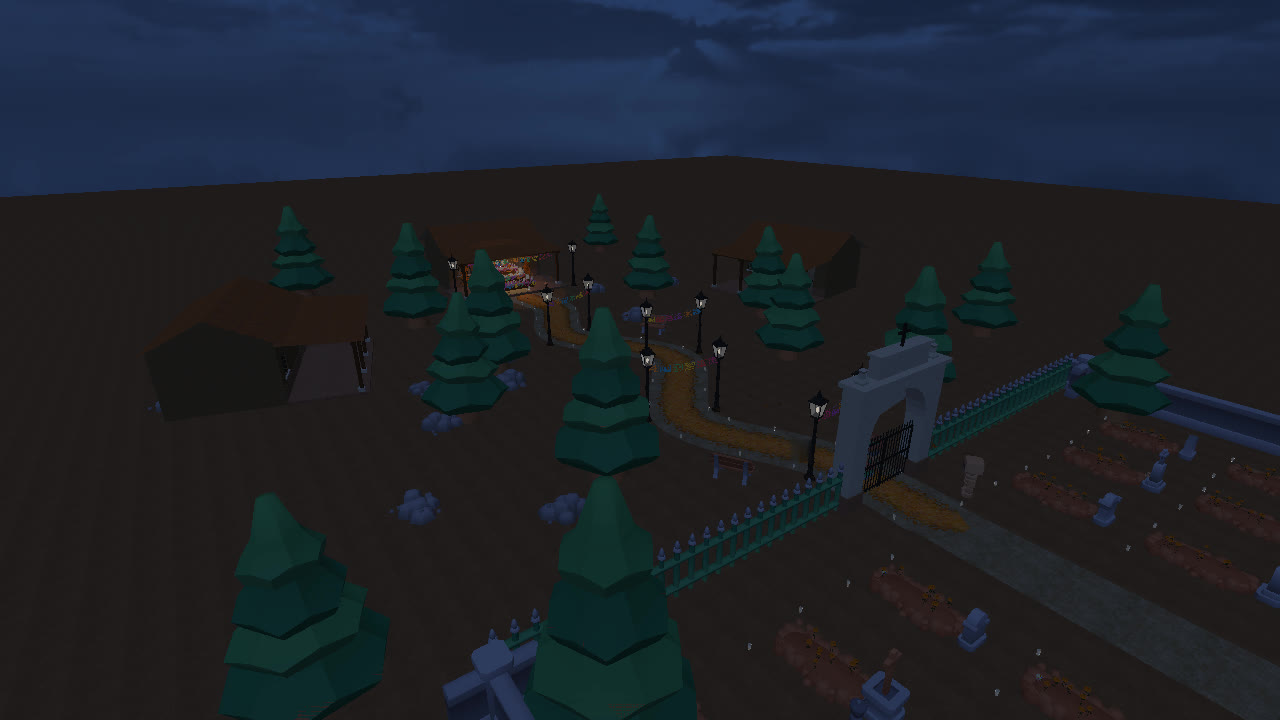
\includegraphics[width=0.85\textwidth]{images/vista-general.jpg}
		\caption{General view: cemetery, petal path, and the house with the offering.}
		\label{fig:general}
	\end{figure}

	\subsection{Texturing, Color, and Lighting}
	The textures of the team-made models were designed with procedural nodes in Blender and baked to color, roughness, and normal maps. In the fragment shader, normals are perturbed without precomputed tangents: the \texttt{dFdx} and \texttt{dFdy} derivatives of position and UV coordinates give the tangent basis of each pixel. Petals and papel picado use alpha clipping to show their outline without extra geometry.

	Lighting combines two techniques:
	\begin{itemize}[leftmargin=*]
		\item \textbf{Phong} for opaque materials: a bluish directional moonlight and up to 25 point lights (votive candles, tall candles, and lanterns) with quadratic attenuation. Specular sharpness is derived from material roughness.
		\item \textbf{Fresnel} for glass and water: Schlick's approximation mixes the transmitted color with a reflection that grows at grazing angles. This is what makes glasses, pitchers, and candle holders readable.
	\end{itemize}
	The environment is a skybox with a cube map. Its vertex shader removes the view translation so the horizon does not move, and its fragment shader darkens the original sunset toward a night tone. To avoid iterating over useless lights, the renderer keeps only the lights whose bounding volume can reach each object and culls primitives outside the camera using frustum planes extracted from the view-projection matrix (Gribb and Hartmann, 2001).

	\subsection{Animation}
	The specification asks for animations of three kinds (basic, keyframe, and procedural) and three media (code, external software, and bones). Table~\ref{tab:animations} relates each animation to its key, medium, and technique. All of them are coordinated by the \texttt{Animaciones} class (\texttt{src/scene/Animaciones.cpp}), which receives the key, advances each animation with the frame time, and writes the result into scene-graph nodes or renderer uniforms.

	\begin{table}[H]
		\centering
		\small
		\begin{tabularx}{\textwidth}{c p{3.3cm} p{2.4cm} X}
			\toprule
			\textbf{Key} & \textbf{Animation} & \textbf{Medium} & \textbf{Technique}\\
			\midrule
			1 & Monarch butterfly & Code & State machine, keyframes on a Catmull-Rom path, and procedural flapping in the body-wing hierarchy. \\
			2 & Camera tour & Code & Seven position and look-at keyframes with smooth interpolation. \\
			3 & Votive candles & Code & On and off states; group-by-group ignition and procedural flicker in GLSL. \\
			4 & Papel picado & Blender & Shape keys baked into a 96-frame vertex cache. \\
			5 & Petal whirlwind & Blender & Keyframes of 720 petals exported as tracks. \\
			6 & Pitcher pouring water & Blender & Keyframes of the pitcher, water level, and stream exported as tracks. \\
			7 & Visitor 1 & Bones & Seven-bone armature; walk, placing the offering, and bow. \\
			8 & Visitor 2 & Bones & Second character; looks at a grave, waves, and dances. \\
			9 & Dancing skeleton & Bones & 12 s dance with five blended steps. \\
			L & Lanterns & Code & Light interaction: gradual switch off and on. \\
			\bottomrule
		\end{tabularx}
		\caption{Available animations and interactions.}
		\label{tab:animations}
	\end{table}

	\subsubsection{Code Animations}
	\textbf{Monarch butterfly (1).} A butterfly rests on the petate in front of the altar. When the key is pressed it goes through the state machine rest, take-off, flight, and landing. The route is defined by ten control points that start at the resting spot, climb in front of the arch, and come back. It is interpolated with the same \texttt{Camino} class used for the path and traversed at constant speed. States are separated by the traveled distance: during the first and last 0.6 m the flapping ramps up or fades, and in the middle stretch it reaches full amplitude. The wings are child nodes of the body, so rotating them around their hinge is enough for them to follow the body's translation and orientation. This is an example of a transformation hierarchy.

	\textbf{Camera tour (2).} Seven position keyframes and seven look-at keyframes describe the entry from the cemetery, the crossing of the gateway, the path, and the arrival at the offering. Both sequences are interpolated with Catmull-Rom and share a time parameter smoothed with $3t^2 - 2t^3$, so the camera starts and stops without jumps. While the tour runs, movement input is ignored; the same key stops it.

	\textbf{Votive candles (3).} A C++ state machine goes through on, switching off, off, and switching on. Each state sets two values sent to the shader: an ignition front along the Z axis and a global level. In GLSL, the \texttt{factorVela} function groups candles into 4.4 m sections. A section lights up when the front reaches it, so candles turn on in groups from the cemetery toward the altar. The same factor adds procedural flicker: two sine waves with a pseudo-random phase per candle. The factor modulates both the flame emission and the point light each candle casts on its surroundings.

	\textbf{Lanterns (L).} The second light interaction gradually brings the emission and light of the lanterns to zero and restores them when pressed again.

	\subsubsection{Animations Created in Blender}
	The three external-software animations were modeled and animated in Blender. For the engine they were baked into data that OpenGL plays back without depending on Blender.

	\textbf{Papel picado (4).} Six sheets are deformed with shape keys (fixed edge, curvature, and wave) animated by keyframes with different phases and amplitudes. The result was baked into a 96-frame vertex cache; each frame the engine copies the positions into the vertex buffer. The key calms or restarts the wind: playback speed goes down or up gradually.

	\textbf{Petal whirlwind (5).} In Blender, a script computed position and rotation keyframes for 720 petals: they lift off the path, swirl in a two-arm spiral in front of the altar, and settle with a sway. The \texttt{exportar\_remolino.py} script reads the scene frame by frame and stores, for each petal, its position, quaternion, and scale in the binary file \texttt{remolino\_petalos.pist}. During the conversion it changes Blender axes ($Z$ up) to OpenGL axes ($Y$ up). In the engine the petals form an instanced batch. Each frame the two neighboring track frames are interpolated and the 720 matrices are rewritten with \texttt{glBufferSubData}.

	\textbf{Pitcher pouring water (6).} The pitcher pivots around its spout. The water inside is clipped by a box whose height is animated so the surface stays level and the volume is preserved; the stream is a curve with an animated bevel; the glass fills through a shape key. The \texttt{exportar\_jarra.py} script exports the pitcher's position and rotation, the water surface height, the glass fill level, and the stream factors. In OpenGL the water clipping becomes a plane: the fragment shader discards fragments with $\mathbf{n}\cdot\mathbf{p} + d > 0$. The stream is a tube whose rings are moved onto the exported curve every frame.

	\subsubsection{Skeletal Animations}
	The characters start from the pieces of the Kenney Graveyard Kit (Kenney, 2021), released under CC0. The \texttt{exportar\_personajes.py} script builds in Blender a seven-bone armature (hips, torso, head, arms, and legs), joins the pieces into one mesh, and binds each piece to its bone. It then generates the clips (idle, walk, walk while carrying, place, stand up, bow, look, wave, short dance, and full dance) and exports each character as a glTF file with a skin and one animation per clip.

	In the engine, \texttt{Modelo::posar} interpolates each bone's translation and rotation tracks (linear and spherical), computes their global matrices, and applies linear blend skinning:
	\begin{equation}
		\mathbf{v}' = \sum_{i} w_i \, G_i \, B_i^{-1} \, \mathbf{v},
	\end{equation}
	where $G_i$ is the bone's global matrix, $B_i^{-1}$ its inverse bind matrix, and $w_i$ the vertex weight. The deformed vertices are uploaded to the mesh buffer and the bounding box is recomputed for frustum culling. Clips are blended over 0.25 s to avoid pose jumps.

	Each character's trajectory is written in code as a sequence of segments (walk along a route, turn, play a clip). While walking, the cycle phase advances with the distance covered (0.95 m per cycle), which keeps the feet from sliding. Visitor 1 carries a pan de muerto attached to an anchor node that is a child of the forearm bone; when the placing clip ends, the bread stays on the first tier of the altar.

	\subsection{Interaction}
	Navigation is first-person, walking or free flight. Table~\ref{tab:controls} lists the controls.

	\begin{table}[H]
		\centering
		\small
		\begin{tabularx}{\textwidth}{p{3.8cm}X}
			\toprule
			\textbf{Input} & \textbf{Action}\\
			\midrule
			W, A, S, D & Walk through the scene. \\
			Shift & Move faster. \\
			Mouse and TAB & Look around; TAB captures or releases the mouse. \\
			F, Q, E & Toggle free flight; go down and up while flying. \\
			Mouse wheel & Adjust movement speed. \\
			1 to 9 & Start the animations in Table~\ref{tab:animations}. \\
			L & Switch the lanterns off or on. \\
			F2 & Toggle solid and wireframe rendering. \\
			R & Return to the cemetery entrance. \\
			Esc & Close the application. \\
			\bottomrule
		\end{tabularx}
		\caption{Application controls.}
		\label{tab:controls}
	\end{table}

	\subsection{Offering Photographs}
	The seven picture frames on the altar are in place, but the photographs are pending for the version the team will present. Each photo is the \texttt{foto} mesh of the frame model. To change it, edit its texture in \path{modelos-blender/portarretratos/portarretratos_texturizados.blend} and export the glTF again; the procedure is in the ``Fotos de la ofrenda'' section of \texttt{README.md}.

	\section{Experiments}

	\subsection{Building on Different Platforms}
	The project was built with CMake on macOS (Xcode), Windows (Visual Studio 2022 and 2026), and Linux (GCC). Tests in earlier deliveries found problems that remain solved in this version:
	\begin{itemize}[leftmargin=*]
		\item Textures were missing outside macOS because image decoding only existed through ImageIO; \texttt{stb\_image} was integrated for Windows and Linux.
		\item On scaled displays the logical window size differs from the framebuffer size. For that reason \texttt{glViewport} receives the size reported by \texttt{glfwGetFramebufferSize}.
		\item \texttt{Rutas.cpp} locates \texttt{assets/} and \texttt{shaders/} from the real executable path, with wide paths on Windows, so the working directory does not matter.
		\item Rounding differences between compilers change the offering piece count by a few units; a small difference is logged as a warning.
		\item The VirtIO driver of a Windows 11 ARM virtual machine did not expose OpenGL 3.3, so the application needs a driver with real OpenGL 3.3 support.
	\end{itemize}

	\subsection{Animation Validation}
	The animations were tested on Linux with Mesa (\texttt{llvmpipe}, OpenGL 4.5 Core) inside a virtual X server. A script outside the repository opened the application at a fixed view, sent the keys with \texttt{xdotool}, and took screenshots at intervals with FFmpeg. This way every animation was checked without manual input. The screenshots in the results section come from those runs. The following was also verified:
	\begin{itemize}[leftmargin=*]
		\item the exported tracks have the expected size: 264 frames $\times$ 720 petals $\times$ 8 values for the whirlwind, and 240 frames $\times$ 13 values for the pitcher;
		\item the pitcher starts 18 cm from the glass, tilts 60° while pouring, and the glass goes from 3\% to 82\% full;
		\item each character has seven joints and all its clips, with the frame length defined in Blender;
		\item visitor 1's bread rests in the front gap of the first tier, without intersecting the sugar skulls or the candles.
	\end{itemize}

	\subsection{Performance}
	Since the engine already filtered lights by bounding volume and culled by frustum, the new animations were designed not to interfere with those mechanisms. The whirlwind updates a single instance buffer per frame. The characters are deformed on the CPU and have a few hundred vertices each. The pitcher only rebuilds the stream tube while it is visible. No animation adds a draw call per animated element.

	\section{Results}

	\subsection{Requirements Compliance}
	Table~\ref{tab:requirements} compares the minimum requirements of the specification with the implementation.

	\begin{table}[H]
		\centering
		\small
		\begin{tabularx}{\textwidth}{p{6.2cm}X}
			\toprule
			\textbf{Requirement} & \textbf{Implementation}\\
			\midrule
			8 library or modeled models & 25 Kenney Graveyard Kit models (graves, crypts, fences, cypresses, characters). \\
			8 team-made models & Over 40 team-made models: altar, arch, flower, petal, candles, bread, sugar skull, papel picado, picture frames, pitcher, glass, lantern, house, gateway, dishes, and sweets. \\
			2 light interactions & Votive candles (3) and lanterns (L). \\
			Skybox and textures on team models & Night cube map and baked textures on every team-made model. \\
			2 skeletal animations & Visitor 1 (7), visitor 2 (8), and dancing skeleton (9). \\
			3 code animations & Butterfly (1), camera tour (2), and candles (3). \\
			3 external-software animations & Papel picado (4), petal whirlwind (5), and pitcher (6). \\
			8 input-driven animations & Nine keys (1 to 9) plus L. \\
			Phong and Fresnel & Phong on opaque materials; Schlick's Fresnel on glass and water. \\
			\bottomrule
		\end{tabularx}
		\caption{Minimum requirements and compliance.}
		\label{tab:requirements}
	\end{table}

	\subsection{Application Screenshots}
	Figures~\ref{fig:cemetery} to \ref{fig:offering} show the main areas of the scene, and Figures~\ref{fig:anim1} to \ref{fig:lanterns} show each animation in progress.

	\begin{figure}[H]
		\centering
		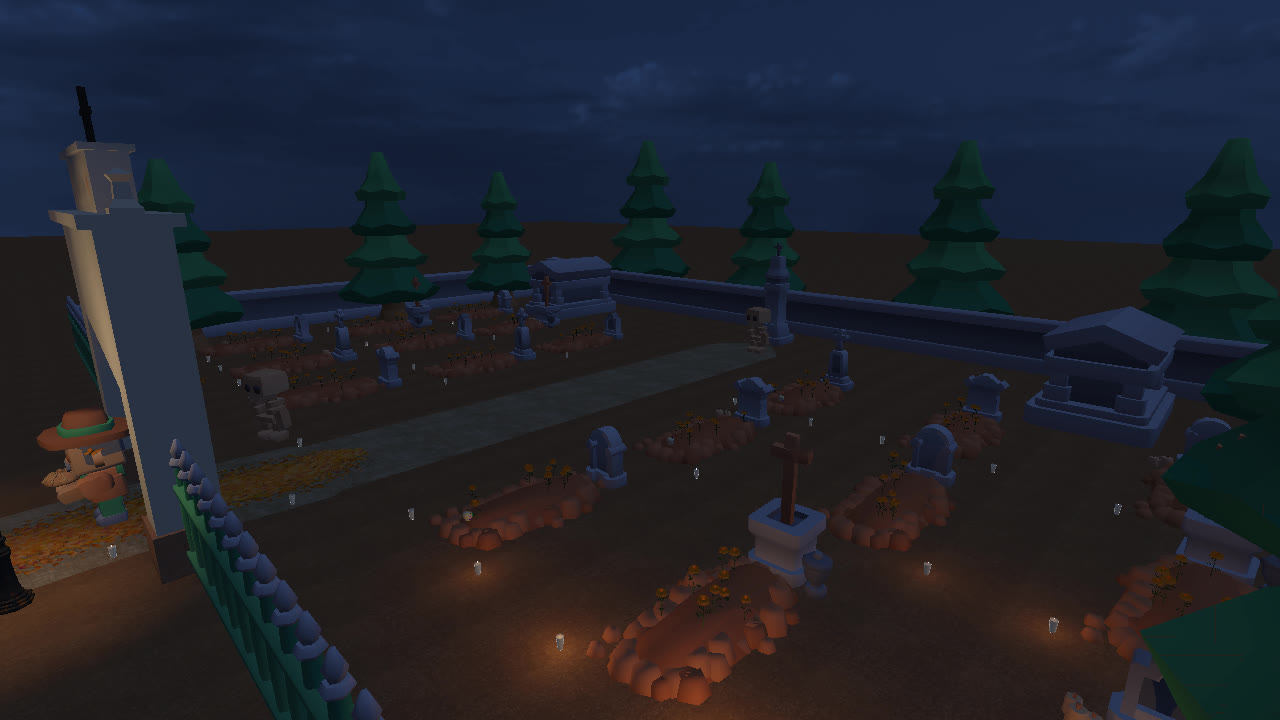
\includegraphics[width=0.85\textwidth]{images/panteon.jpg}
		\caption{Cemetery with graves, crypts, and cypresses from the library.}
		\label{fig:cemetery}
	\end{figure}

	\begin{figure}[H]
		\centering
		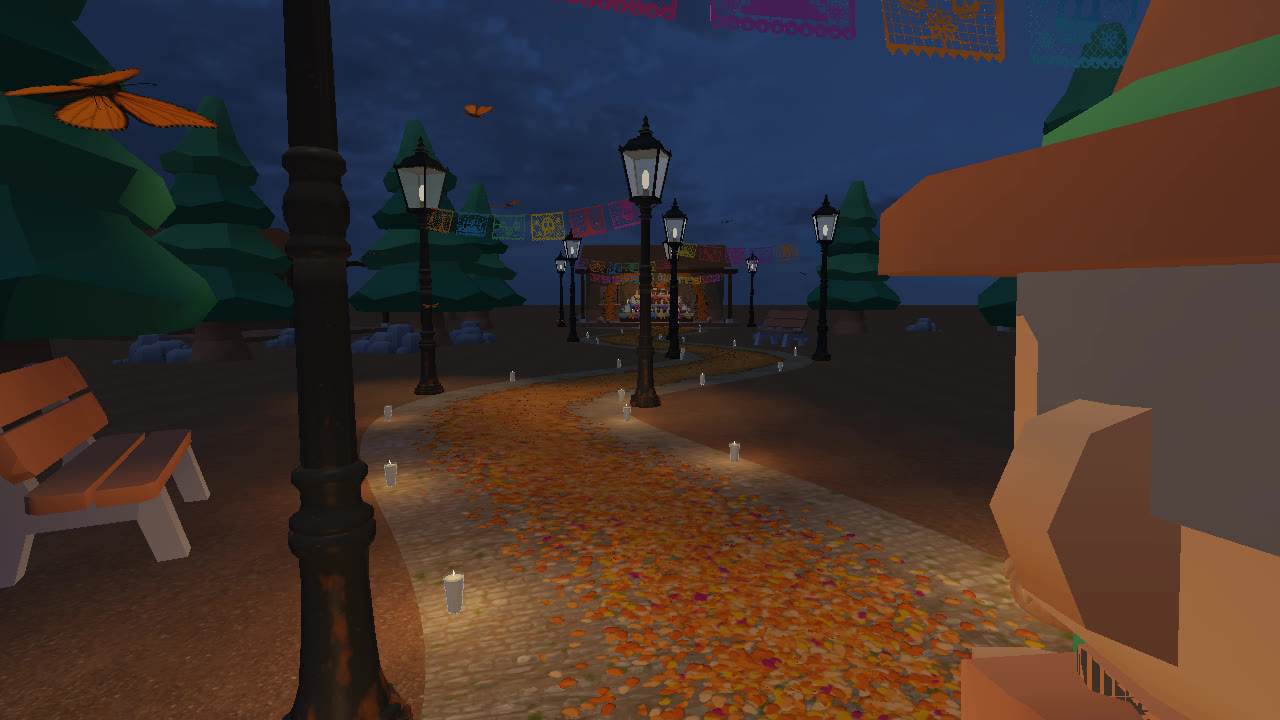
\includegraphics[width=0.85\textwidth]{images/camino.jpg}
		\caption{Petal path with votive candles, lanterns, and papel picado.}
		\label{fig:path}
	\end{figure}

	\begin{figure}[H]
		\centering
		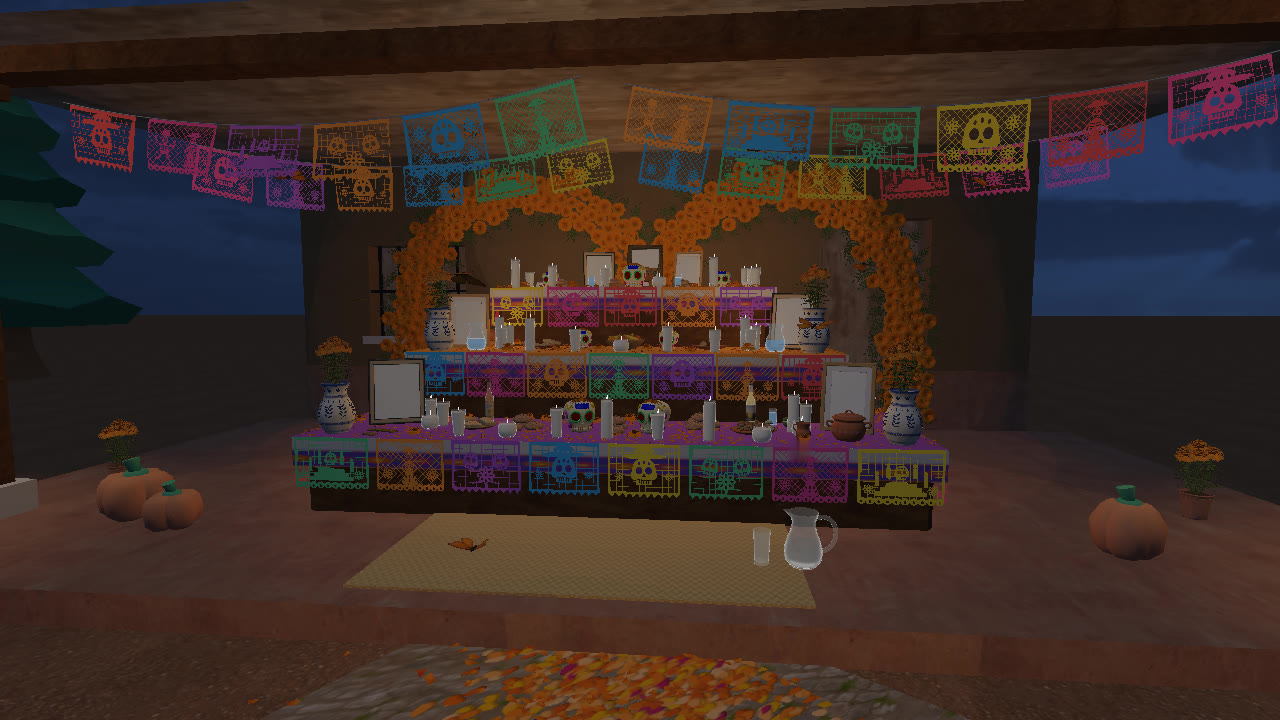
\includegraphics[width=0.85\textwidth]{images/ofrenda.jpg}
		\caption{Three-tier offering in the porch of the adobe house.}
		\label{fig:offering}
	\end{figure}

	\begin{figure}[H]
		\centering
		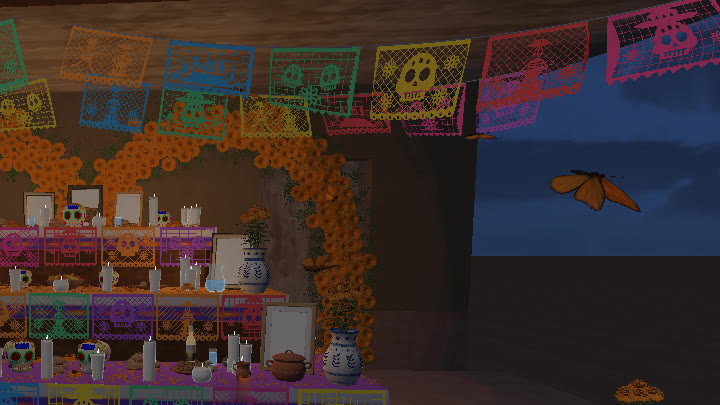
\includegraphics[width=0.85\textwidth]{images/anim-1-mariposa.jpg}
		\caption{Animation 1: the monarch butterfly in flight in front of the altar.}
		\label{fig:anim1}
	\end{figure}

	\begin{figure}[H]
		\centering
		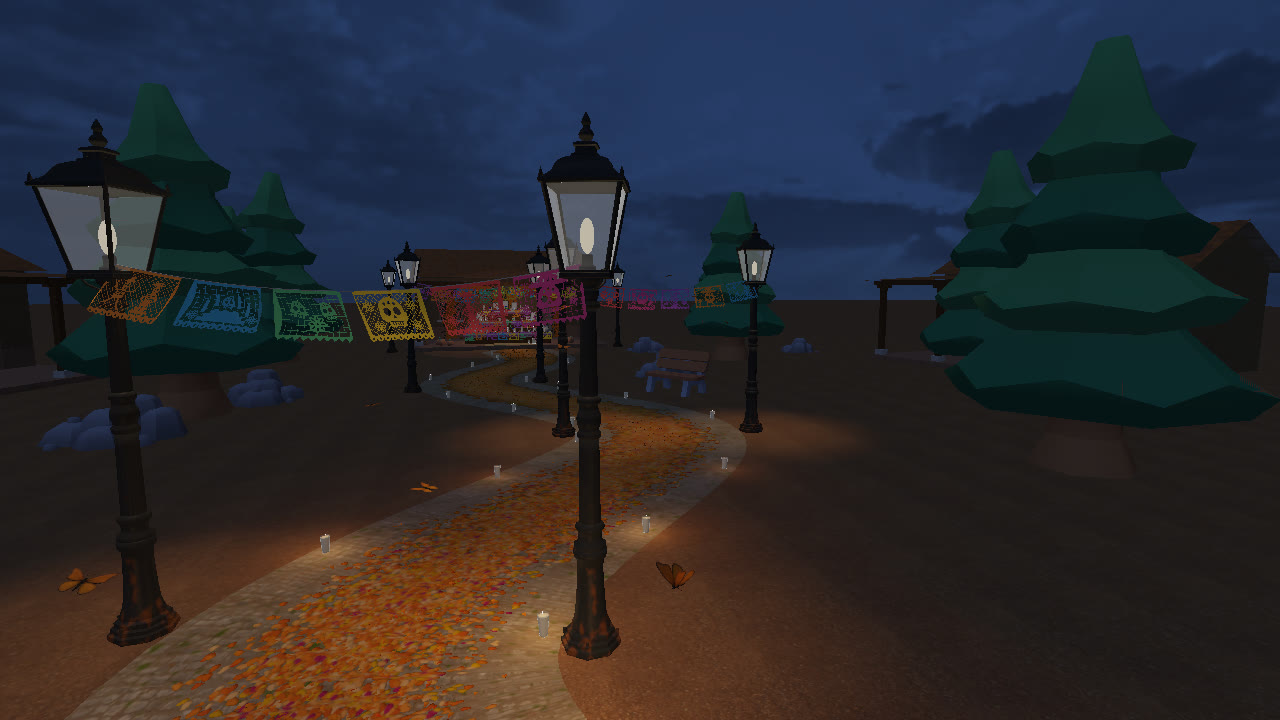
\includegraphics[width=0.85\textwidth]{images/anim-2-recorrido.jpg}
		\caption{Animation 2: an intermediate frame of the camera tour along the path.}
		\label{fig:anim2}
	\end{figure}

	\begin{figure}[H]
		\centering
		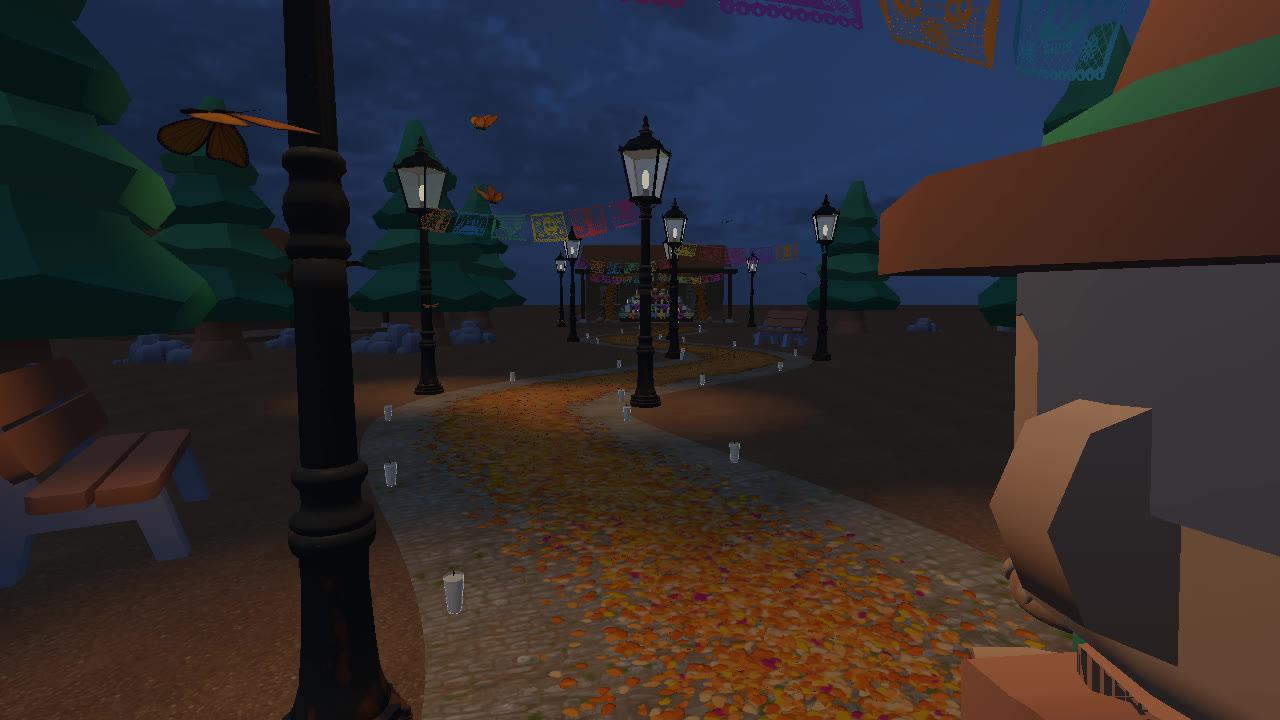
\includegraphics[width=0.49\textwidth]{images/anim-3-veladoras-a.jpg}\hfill
		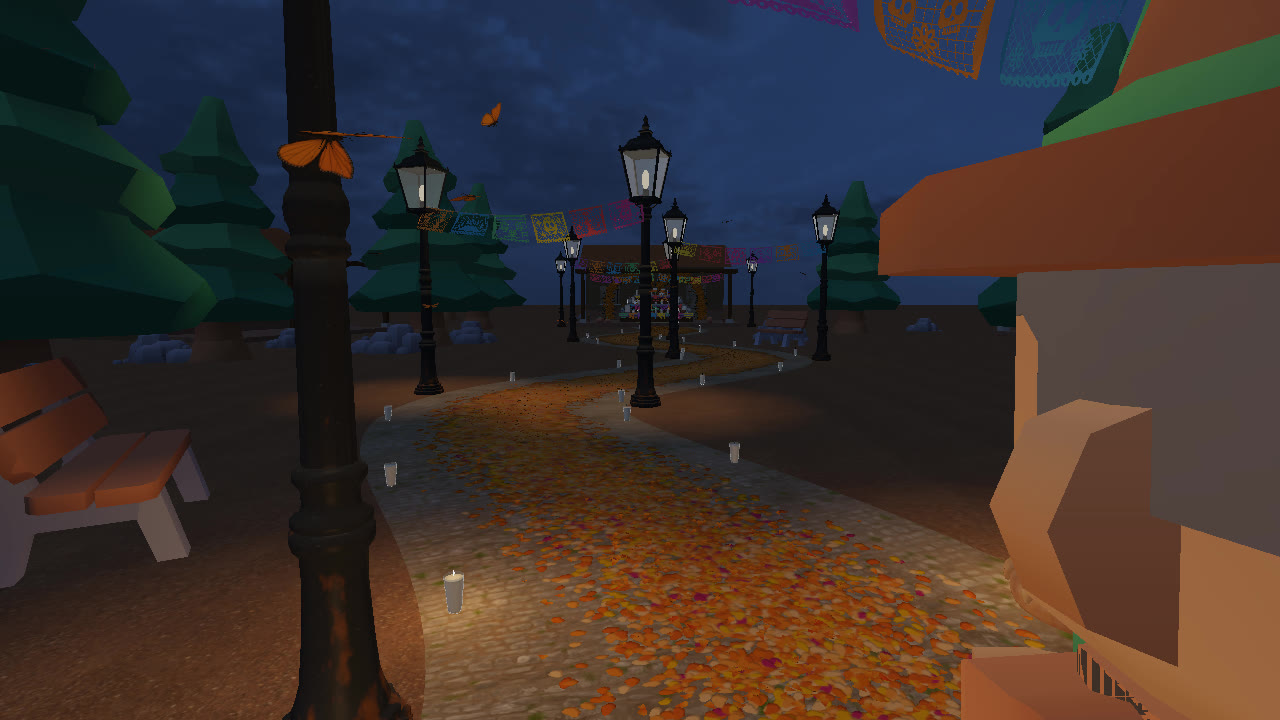
\includegraphics[width=0.49\textwidth]{images/anim-3-veladoras-b.jpg}
		\caption{Animation 3: candles off (left) and lighting up in groups (right).}
		\label{fig:anim3}
	\end{figure}

	\begin{figure}[H]
		\centering
		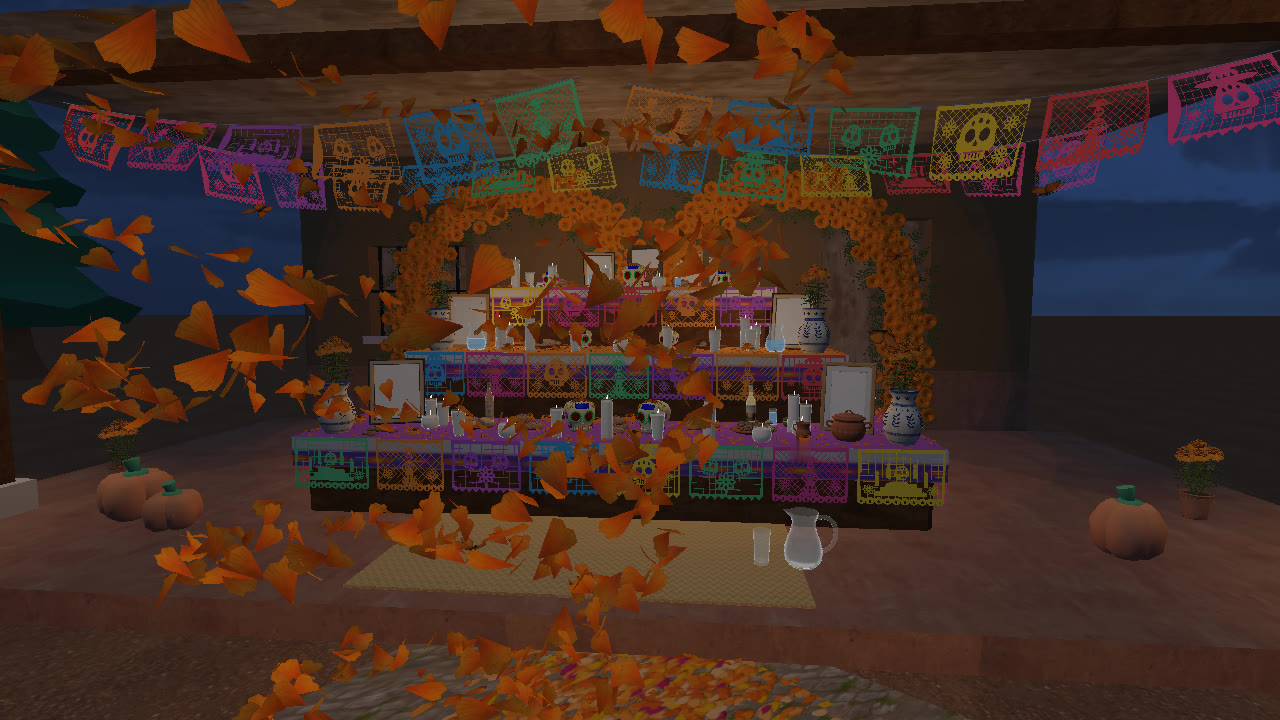
\includegraphics[width=0.85\textwidth]{images/anim-5-remolino.jpg}
		\caption{Animation 5: the petals form the spiral in front of the offering.}
		\label{fig:anim5}
	\end{figure}

	\begin{figure}[H]
		\centering
		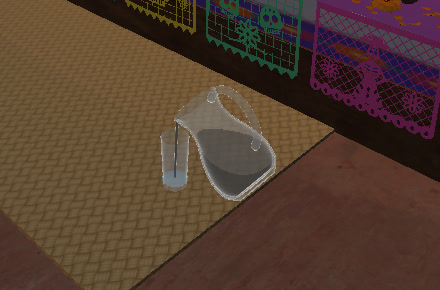
\includegraphics[width=0.6\textwidth]{images/anim-6-jarra.jpg}
		\caption{Animation 6: the pitcher pours water into the glass on the petate.}
		\label{fig:anim6}
	\end{figure}

	\begin{figure}[H]
		\centering
		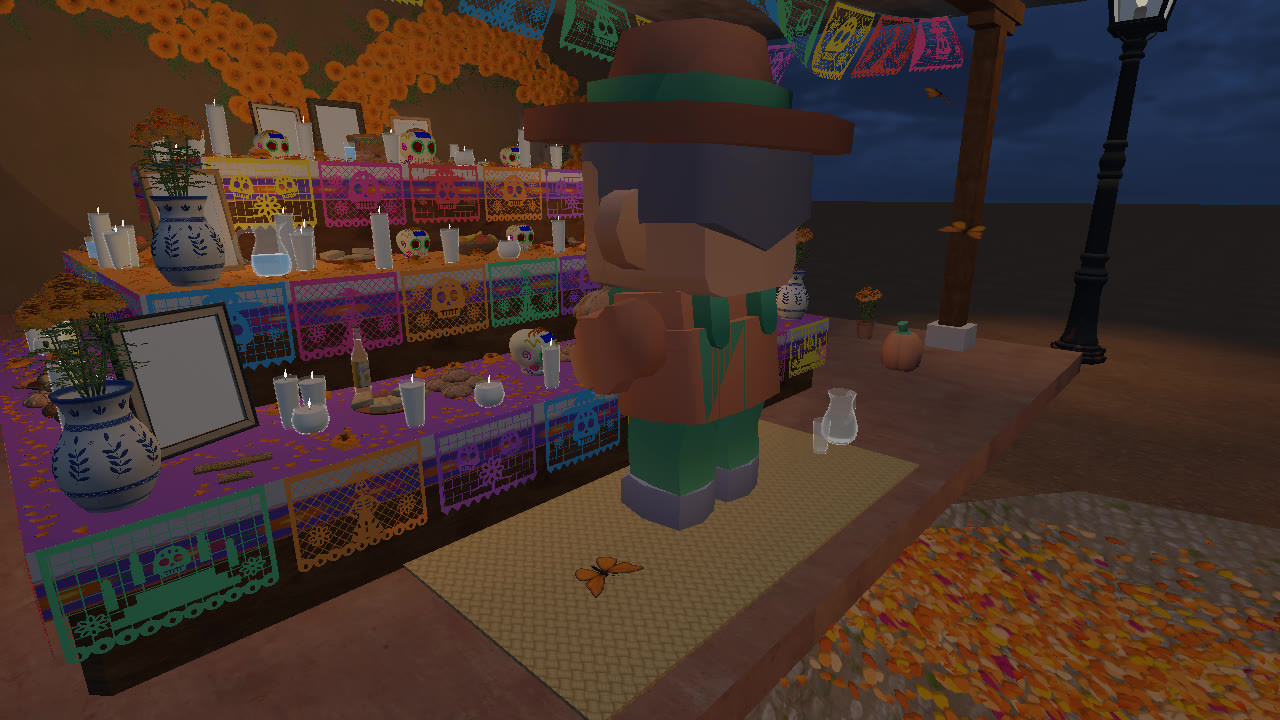
\includegraphics[width=0.85\textwidth]{images/anim-7-visitante.jpg}
		\caption{Animation 7: the visitor leaves the pan de muerto on the first tier of the altar.}
		\label{fig:anim7}
	\end{figure}

	\begin{figure}[H]
		\centering
		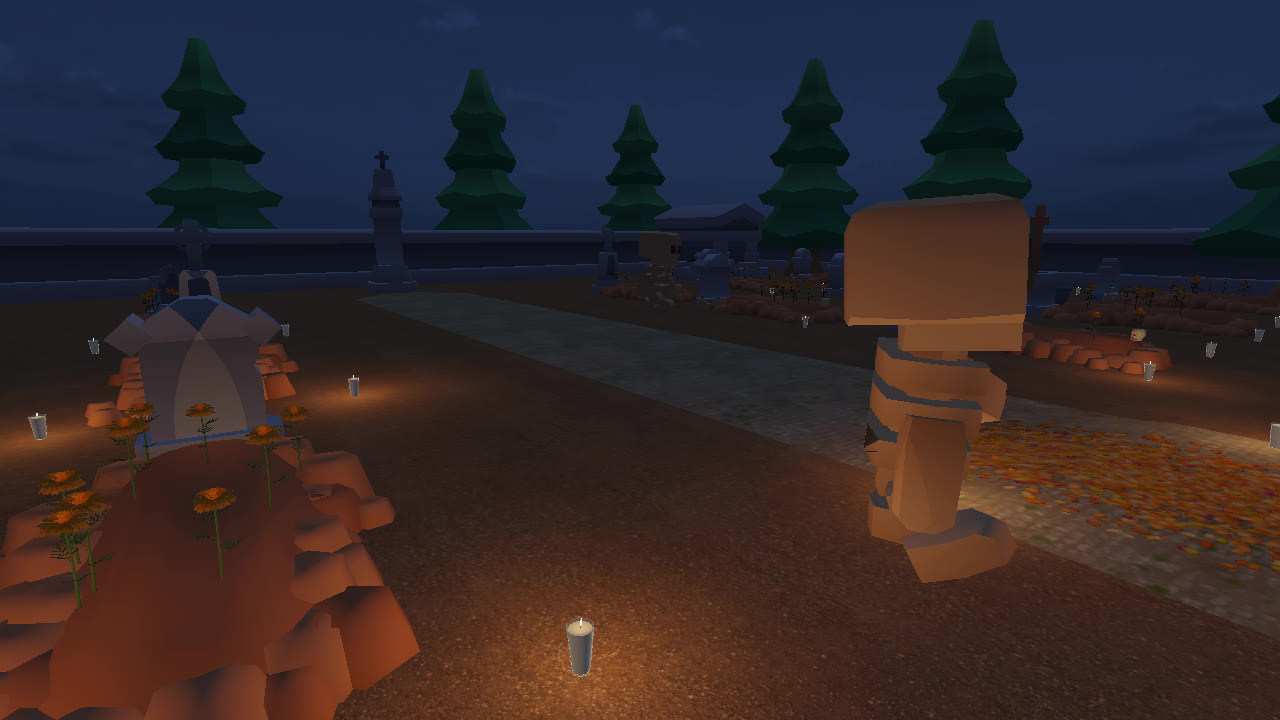
\includegraphics[width=0.85\textwidth]{images/anim-8-9-panteon.jpg}
		\caption{Animations 8 and 9: visitor 2 walks through the cemetery while the skeleton dances by the gateway.}
		\label{fig:anim8}
	\end{figure}

	\begin{figure}[H]
		\centering
		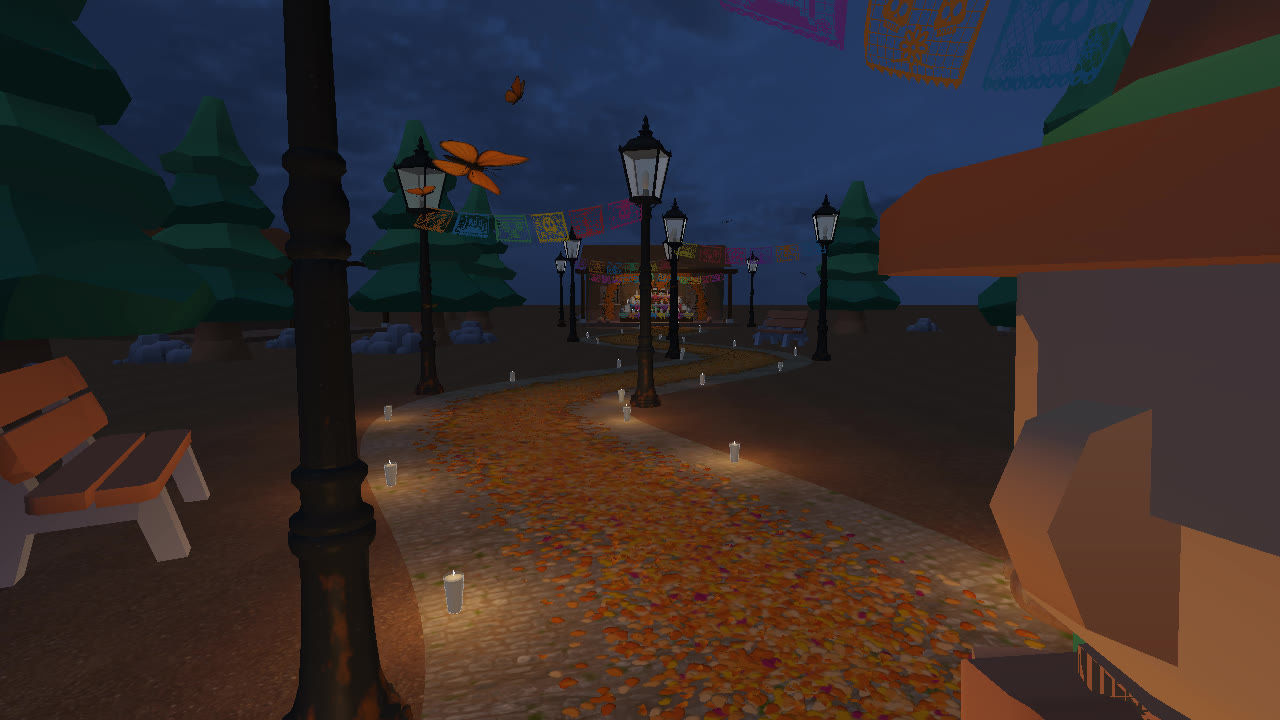
\includegraphics[width=0.85\textwidth]{images/faroles-apagados.jpg}
		\caption{Interaction L: the path with the lanterns off; only the votive candles remain.}
		\label{fig:lanterns}
	\end{figure}

	\section{Individual Conclusions}

	\subsection*{Basilio Illescas Andrés}
	\textit{To be written by the team member.}

	\subsection*{Cruz Macedo Samuel Santiago}
	\textit{To be written by the team member.}

	\subsection*{Pérez Olvera Alexis Abraham}
	\textit{To be written by the team member.}

	\subsection*{Trejo Olvera Emmanuel}
	\textit{To be written by the team member.}

	\section{Demo Video}
	Link to the 3 to 5 minute video: \textit{(to be added)}.

	\section{References}
	\begin{itemize}[leftmargin=*]
		\item Akenine-Möller, T., Haines, E., Hoffman, N., Pesce, A., Iwanicki, M., \& Hillaire, S. (2018). \textit{Real-time rendering} (4th ed.). CRC Press.
		\item Barry, P. J., \& Goldman, R. N. (1988). A recursive evaluation algorithm for a class of Catmull-Rom splines. \textit{ACM SIGGRAPH Computer Graphics, 22}(4), 199--204. \url{https://doi.org/10.1145/378456.378511}
		\item Blender Foundation. (2026). \textit{Blender 5.2 manual}. \url{https://docs.blender.org/manual/en/latest/}
		\item Catmull, E., \& Rom, R. (1974). A class of local interpolating splines. In R. E. Barnhill \& R. F. Riesenfeld (Eds.), \textit{Computer aided geometric design} (pp. 317--326). Academic Press.
		\item Gregory, J. (2018). \textit{Game engine architecture} (3rd ed.). CRC Press.
		\item Gribb, G., \& Hartmann, K. (2001). \textit{Fast extraction of viewing frustum planes from the world-view-projection matrix}. \url{https://www.gamedevs.org/uploads/fast-extraction-viewing-frustum-planes-from-world-view-projection-matrix.pdf}
		\item Kenney. (2021). \textit{Graveyard kit} [3D models, CC0 license]. \url{https://kenney.nl/assets/graveyard-kit}
		\item Khronos Group. (2021). \textit{glTF 2.0 specification}. \url{https://registry.khronos.org/glTF/specs/2.0/glTF-2.0.html}
		\item Magnenat-Thalmann, N., Laperrière, R., \& Thalmann, D. (1988). Joint-dependent local deformations for hand animation and object grasping. In \textit{Proceedings of Graphics Interface '88} (pp. 26--33). Canadian Information Processing Society.
		\item Phong, B. T. (1975). Illumination for computer generated pictures. \textit{Communications of the ACM, 18}(6), 311--317. \url{https://doi.org/10.1145/360825.360839}
		\item Schlick, C. (1994). An inexpensive BRDF model for physically-based rendering. \textit{Computer Graphics Forum, 13}(3), 233--246. \url{https://doi.org/10.1111/1467-8659.1330233}
		\item Segal, M., \& Akeley, K. (2010). \textit{The OpenGL graphics system: A specification (version 3.3, core profile)}. Khronos Group. \url{https://registry.khronos.org/OpenGL/specs/gl/glspec33.core.pdf}
		\item Shoemake, K. (1985). Animating rotation with quaternion curves. \textit{ACM SIGGRAPH Computer Graphics, 19}(3), 245--254. \url{https://doi.org/10.1145/325165.325242}
		\item UNESCO. (2008). \textit{Indigenous festivity dedicated to the dead}. Intangible Cultural Heritage. \url{https://ich.unesco.org/en/RL/indigenous-festivity-dedicated-to-the-dead-00054}
		\item Yuksel, C., Schaefer, S., \& Keyser, J. (2011). Parameterization and applications of Catmull-Rom curves. \textit{Computer-Aided Design, 43}(7), 747--755. \url{https://doi.org/10.1016/j.cad.2010.08.008}
	\end{itemize}
\end{document}
